\subsection{The Langevin Equation}
\begin{equation}
	{\LARGE{{m \frac{dv}{dt} = -\lambda v + \eta(t)}}}
	\label{eq:1}
\end{equation}
\subsection{Terms of the Equation}

{\normalsize{In the above equation,}}\\
{\normalsize {\textbf{m} denotes the mass of the particle }}\\
{\normalsize {\textbf{$ \lambda $ } represents the viscous force }}\\
{\normalsize {\textbf{v} represents the velocity of the particle }}\\
{\normalsize {\textbf{$  \eta (t)$} is the \textit{noise term} which describes the force}}\\

\subsection{Description}

{\normalsize {The Langevin Equation is used to describe \textit{Brownian Motion}.}\\
{\normalsize {Brownian motion is the observed random movement that is portrayed by a particle when in a fluid due to its collisions with the other molecules.}}\\ 

{\normalsize {The Langevin equation is a phenomenological stochastic differential equation of motion (see Equation \ref{eq:1}). It describes the time evolution of a subset of the various degrees of freedom where it slowly relaxes the macroscopic variables and rapidly relaxes the microscopic variables. Thus, the equation is stochastic in nature. \cite{para2}
\begin{figure}[h]
	\centerline{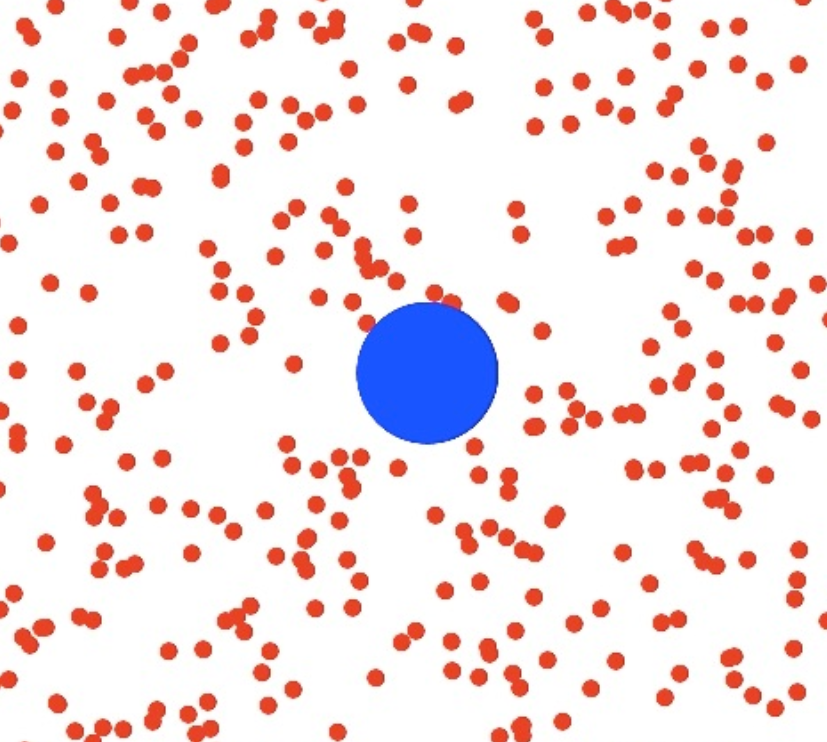
\includegraphics[width=4cm]{mm20b057.PNG}}
	\caption{Brownian Motion}
        \label{fig:1}
\end{figure} \cite{pic}

Brownian motion (see Figure \ref{fig:1}) is by far the simplest way to approximate the dynamics of the particles of a non equilibrium system. In the given equation, the net force has been split into a systematic part \textit{(friction)} and a fluctuating part \textit{(noise)}. Both these forces arise due to the interaction of the Brownian particle with the environment. \cite{para3}
}}



\subsection{Importance}
\normalsize{The original Langevin equation helps you describe the Brownian motion of the given Brownian particle, but the application of this equation sees no boundaries. Various forms of this equation has been used in electrical resistors, critical dynamics, harmonic oscillators in a fluid, to find trajectories of Brownian particles and in Boltzmann statistics.} \cite{imp}

